\documentclass[a4paper,11pt]{article}

\usepackage[utf8]{inputenc} \usepackage[T1]{fontenc}
\usepackage{fancyhdr} \usepackage{graphicx,subfig} \usepackage{lastpage}
\usepackage{amssymb,amsmath} \usepackage{siunitx} \usepackage[nodayofweek]{datetime}
\usepackage[top=3.5cm,bottom=2.5cm,left=3cm,right=3cm,headheight=40pt]{geometry}
\usepackage{parskip} \usepackage{float} \usepackage{enumitem} \pagestyle{fancy}
\usepackage[colorlinks=true,allcolors=blue]{hyperref} \hypersetup{
	pdfauthor={Michaël Defferrard},
	pdftitle={Project stage 1: Terrain generation},
	pdfsubject={Introduction to Computer Graphics}
}

\lhead{Introduction to Computer Graphics\\Project stage 1: Terrain generation\\Group 19}
\chead{\hspace{2.5cm}EPFL\\\hspace{2.5cm}\shortdate\today\\\hspace{2.5cm}\thepage/\pageref{LastPage}}
\rhead{Michaël \textsc{Defferrard}\\Pierre \textsc{Fechting}\\Vu Hiep \textsc{Doan}}
\cfoot{}

\begin{document}


\section{Overview}

This report presents our advancement on the first part of the project : terrain generation using procedural methods. Figure~\ref{teaser} shows an example of what our actual code base is able to generate. All the minimal steps to display a procedurally generated terrain were successfully completed. We did not yet have the time to implement more advanced methods. We however plan to do so.

\begin{figure}[ht]
	\centering
	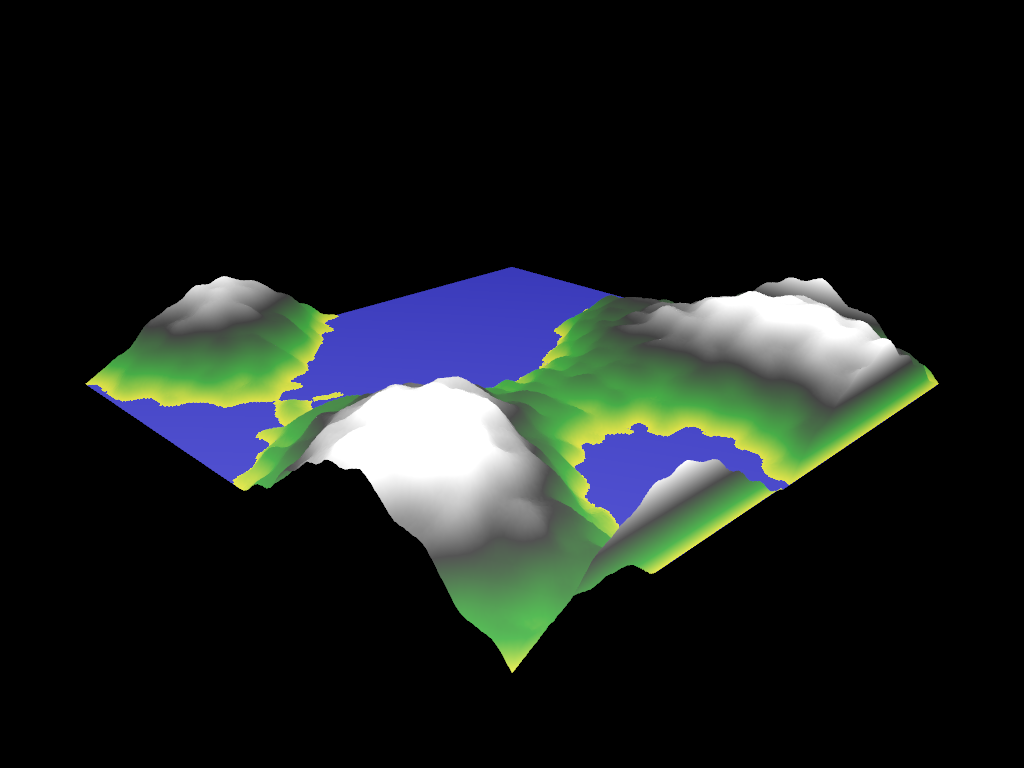
\includegraphics[height=7cm]{{{img_stage1/fBm_1.1_10.0_10_2.0_withZeroGrad_seed10}}}
	\caption{Example terrain generated by fractal Brownian motion with $H=1.1$, $l=10$ and 10 octaves, Perlin basis noise function.}
	\label{teaser}
\end{figure}

The main difficulties we did encounter during this first stage were about the framework. As for practicals and homeworks everything was set, we did not have any experience on the various functions used to create, bind or copy data into the various OpenGL object types. We took a lot of time to figure out how all this was working together. Now that we acquired some experience, the implementation of the next steps will surely be facilitated.

We did also loose time with some oddities. Let us give an example. The Perlin noise permutation table contains values from 0 to 255. It would thus make sense to store them as a \texttt{GL\_ubyte} array and to pass them to the shaders as a 1D texture of internal type \texttt{GL\_R8UI}. No data were however passed. The glsl \texttt{textureSize} built-in function was always returning a size of 0. After hours of trying to understand why a simple buffer copy does not work, we found a little note which said that standard compliant implementations do not have to exactly match the provided list of internal types and can fall back to other types\footnote{Explained on the OpenGL \href{https://www.opengl.org/wiki/GLAPI/glTexImage1D}{wiki}.}. After trying some other types like \texttt{GL\_R32I} we resigned and used \texttt{GL\_R32F} at the expense of 2 bytes per texel. The exact cause of this problem was however not elucidated.

As noted in the hand-out, we add to the fact that OpenGL debugging is hard and time-consuming. We use a lot of "black box" functions and debugging is not very practical. This is especially true for glsl and the infrastructure for data passing, as there is nothing until it works. At least at the beginning. When the infrastructure is in place and an output buffer is available, "printf debugging" can be used.

%We use git\footnote{the distributed revision control system} to manage our sources. Some members of the team were not familiar with source code management tools. It was a great to


\section{Implementation}

\subsection{Triangle grid}

We first generate the flat triangle mesh as a base for our terrain. The implementation is quite straightforward for a grid of size $N \times N$ as first, two VBOs storing the positions of each vertex and the corresponding faces' indices also are calculated.

We then render it as a triangle mesh by function \texttt{glDrawElements} to get a smooth triangle mesh (see 		~\ref{triangle_grid_full}). It is also worth noticing the use of \texttt{glPolygonMode}, which allows us to render only the triangles' boundaries as shown in figures~\ref{triangle_grid_8}, \ref{triangle_grid_16} and~\ref{triangle_grid_64} for $N=8$, $N=16$ and $N=64$, respectively.

\begin{figure}[ht]
	\centering
	\subfloat[Lines with $N=8$]{
		\label{triangle_grid_8}
		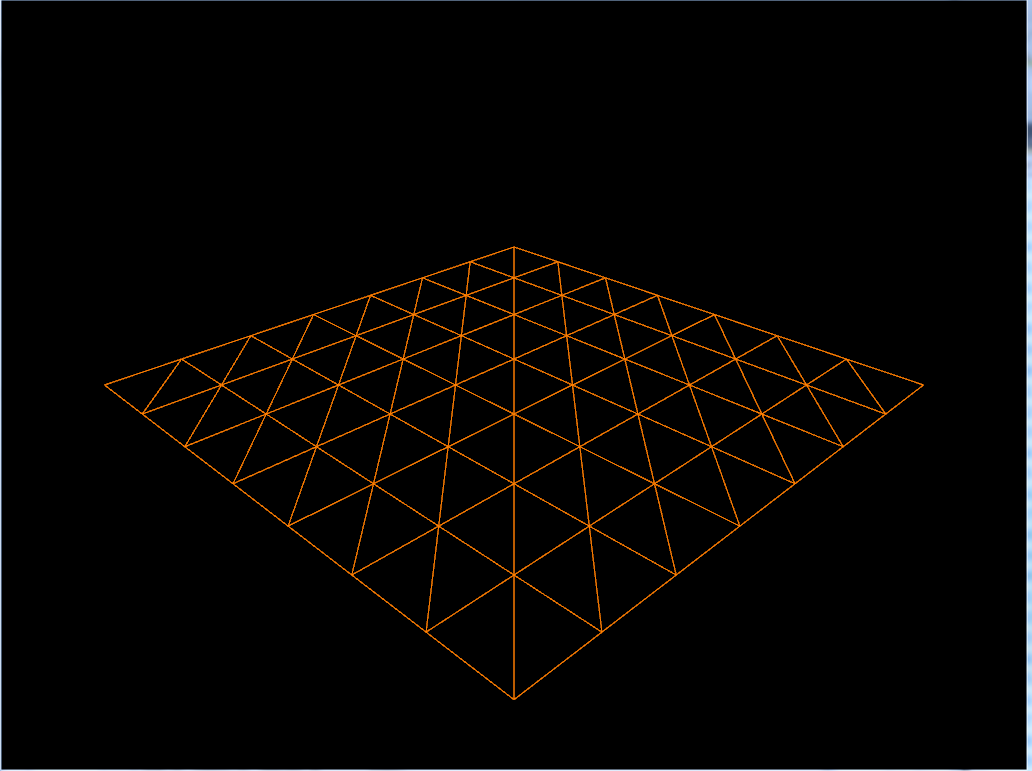
\includegraphics[height=4cm]{{{img_stage1/triangle_grid_8}}}
	} \quad
	\subfloat[Lines with $N=16$]{
		\label{triangle_grid_16}
		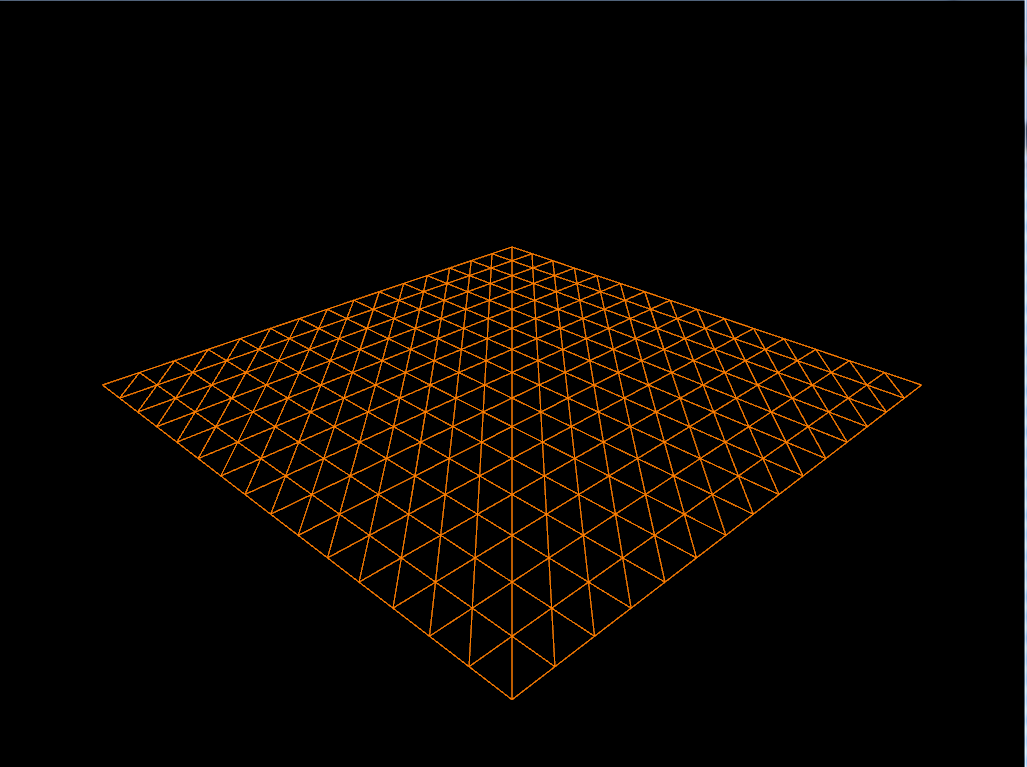
\includegraphics[height=4cm]{{{img_stage1/triangle_grid_16}}}
	} \quad
	\subfloat[Lines with $N=64$]{
		\label{triangle_grid_64}
		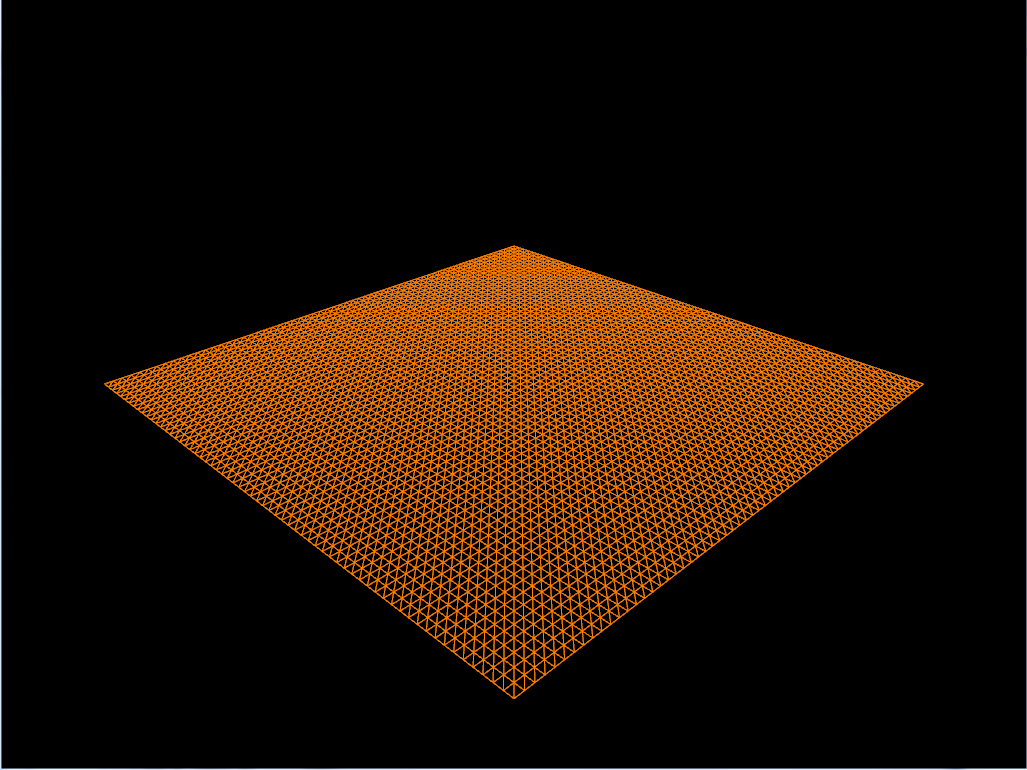
\includegraphics[height=4cm]{{{img_stage1/triangle_grid_64}}}
	} \quad
	\subfloat[Triangles]{
		\label{triangle_grid_full}
		
\includegraphics[height=4cm]{{{img_stage1/triangle_grid_full}}}
	}
	\caption{Triangle grid}
	\label{triangle_grid}
\end{figure}

\subsection{Diffuse shading}

The terrain generated from displacing each vertex in base triangle grid according to height map will be applied the diffuse shading for better visualization. In short, each vertex will be colored by the result value of following equation: $I_dk_d(N\cdot L)$ where $I_d$ and $k_d$ is the diffuse color of the light source and material, respectively. $N$ is the normal vector at that vertex and $L$ is the normalized light direction vector.

We define te diffuse color of light source and material as well as the light position so except $N$, other values are very easy to compute. For calculating normal vector $N$, we use finite difference to approximate a gradient vectors $\nabla x$ and $\nabla y$ along \textit{x} and \textit{y} directions. Note that to compute theses gradients, we need the elevation at four neighboring vertices as well, which can be done again by looking up on the height map that we generated.

Then, the normal vector will be cross product of $\nabla x$ and $\nabla y$. 

\subsection{Heightmap texture}

We did first construct an heightmap by hand (\texttt{gen\_test\_height\_map}) with a 3x3 pixels texture to test the displacement procedure of the rendering vertex shader and the height sensible coloring of the rendering fragment shader (fig.~\ref{test_heightmap}). We then implemented the texture rendering (\texttt{gen\_height\_map}). To test the framework, we rendered a simple texture of 1024x1024 pixels which all have the value of 0.5 (fig.~\ref{test_heightmap_gen}).

\begin{figure}[ht]
	\centering
	\subfloat[Heightmap constructed by hand]{
		\label{test_heightmap}
		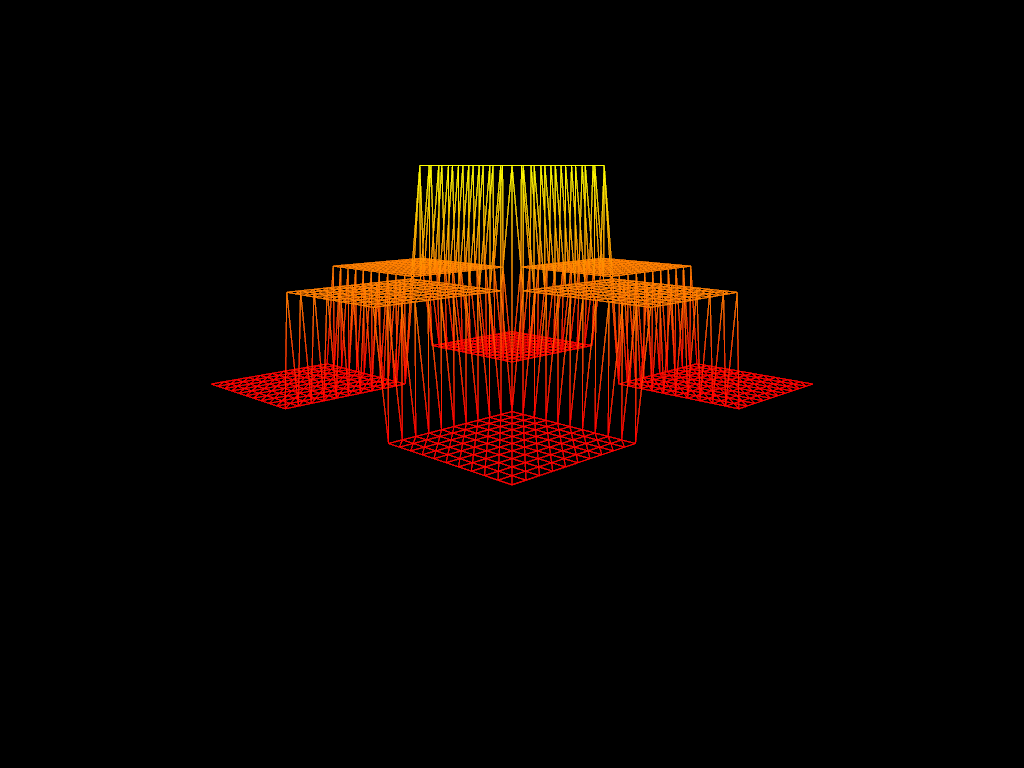
\includegraphics[height=4cm]{{{img_stage1/test_heightmap}}}
	} \quad
	\subfloat[Simple generated heightmap]{
		\label{test_heightmap_gen}
		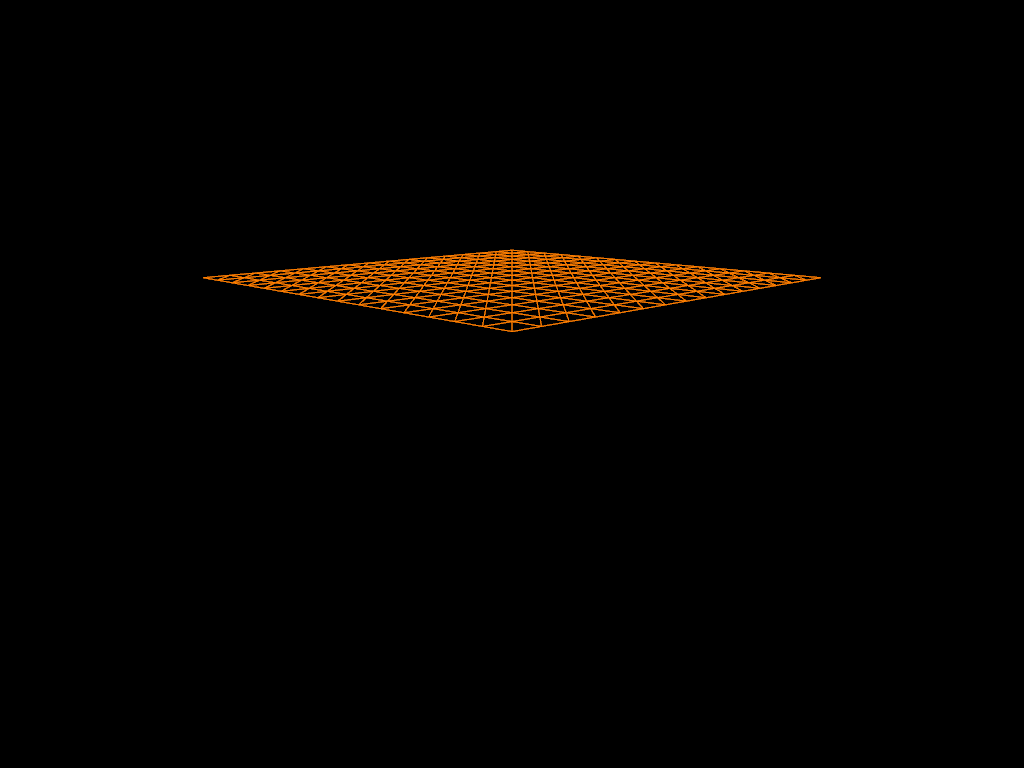
\includegraphics[height=4cm]{{{img_stage1/test_heightmap_gen}}}
	}
	\caption{Heightmaps}
\end{figure}

\subsection{Perlin noise}

We then implemented the Perlin noise in the heightmap fragment shader. As suggested by the tutorial\footnote{The GPU Gems 2 \href{http://http.developer.nvidia.com/GPUGems2/gpugems2_chapter26.html}{tutorial} given in the hand-out}, we used a permutation table to generate a pseudo-random number per square.

indexed texture access instead of interpolation in normalize coordinates

Show some screenshots with different frequencies and amplitudes of the noise function.

With / without zeros in gradients.

Fisher-Yates / Knuth shuffle is unbiased, as long as the underlying random generator is. (page note to wikipedia)

texelFetch instead of interpolation

\subsection{Fractal Brownian movement}

\begin{figure}[ht]
	\centering
	\subfloat[Seed of 2]{
		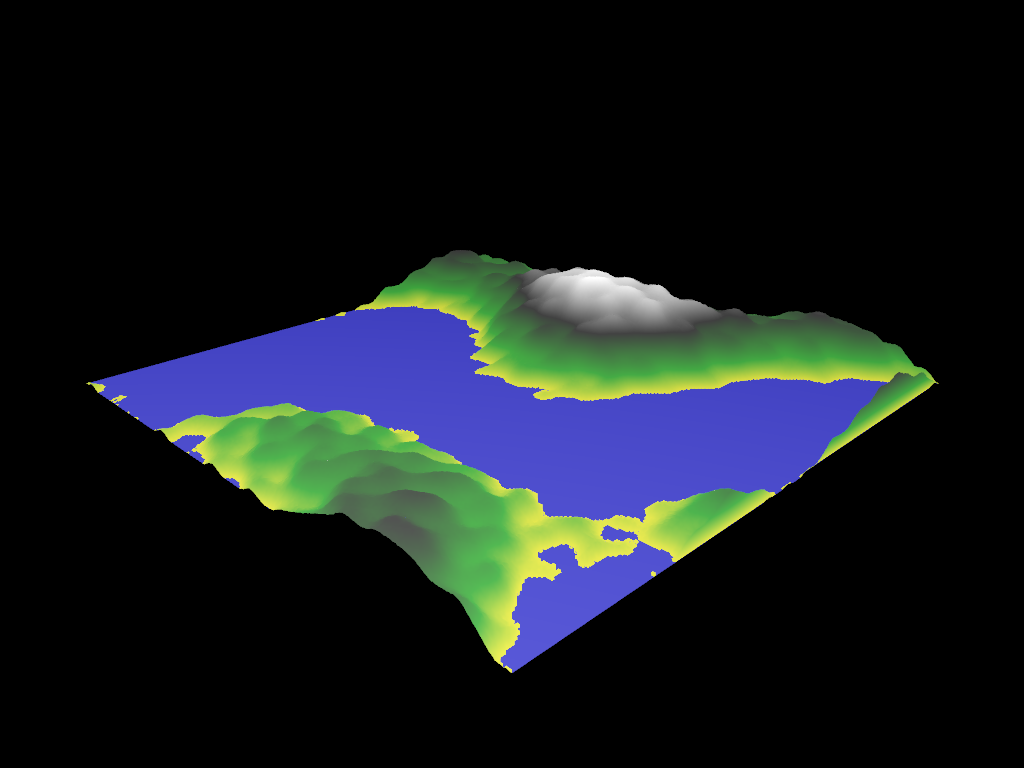
\includegraphics[height=3cm]{{{img_stage1/fBm_1.1_10.0_10_2.0_withZeroGrad_seed2}}}
	} 
	\subfloat[Seed of 3]{
		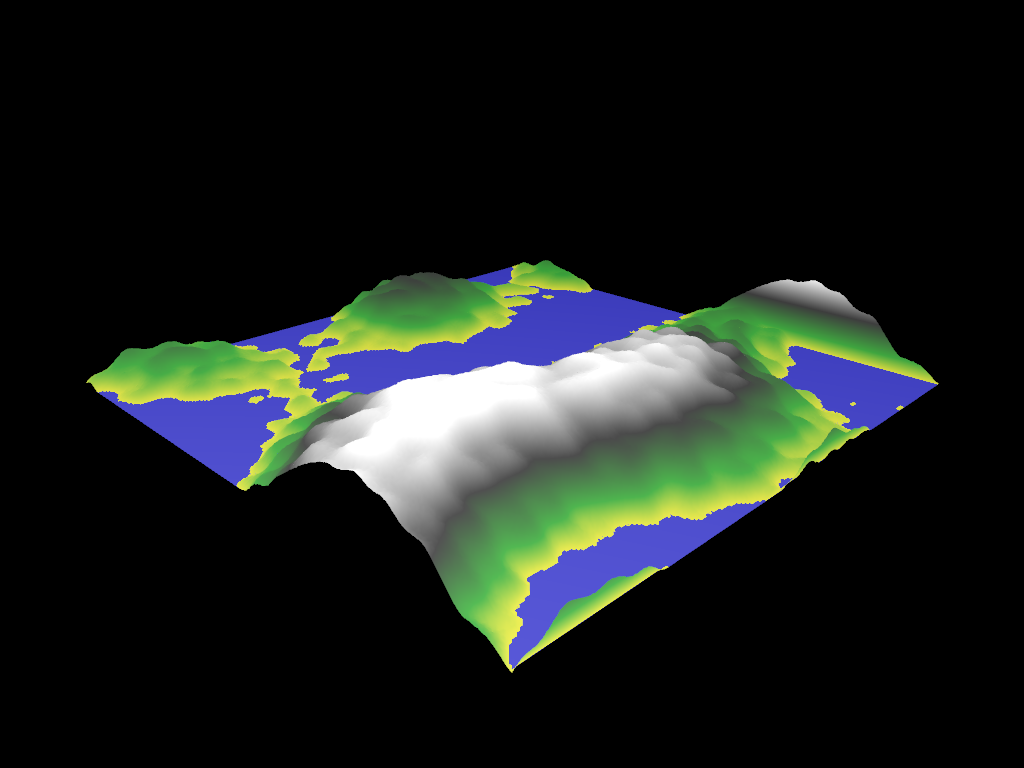
\includegraphics[height=3cm]{{{img_stage1/fBm_1.1_10.0_10_2.0_withZeroGrad_seed3}}}
	} 
	\subfloat[Seed of 4]{
		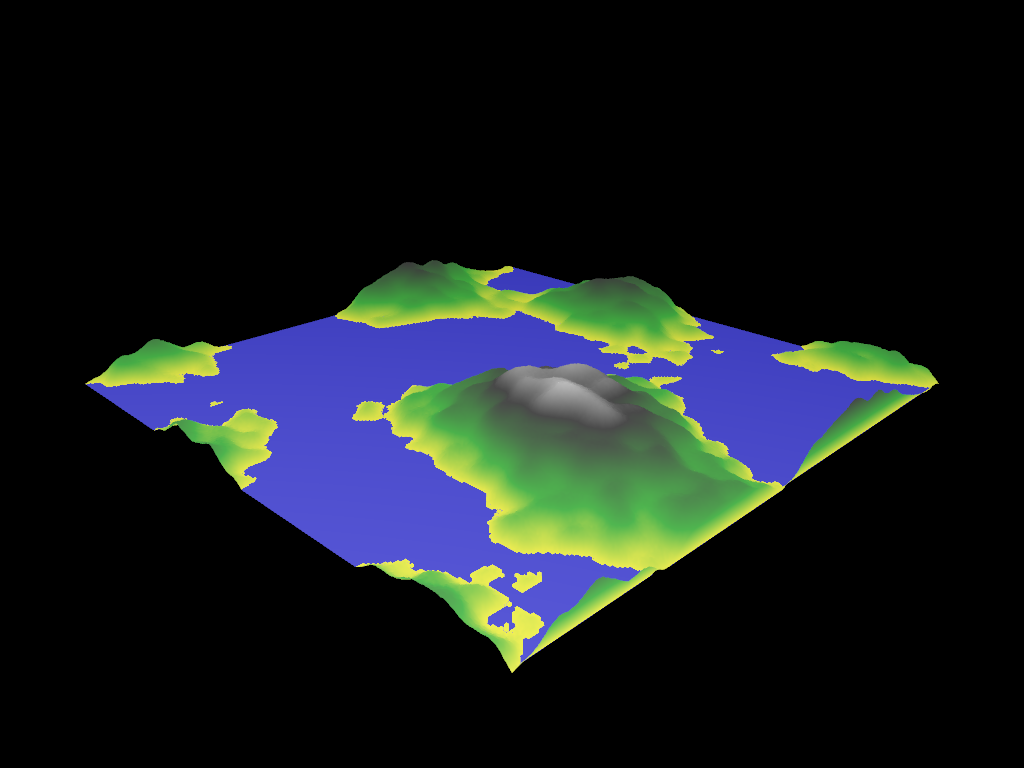
\includegraphics[height=3cm]{{{img_stage1/fBm_1.1_10.0_10_2.0_withZeroGrad_seed4}}}
	} \\
	\subfloat[Seed of 5]{
		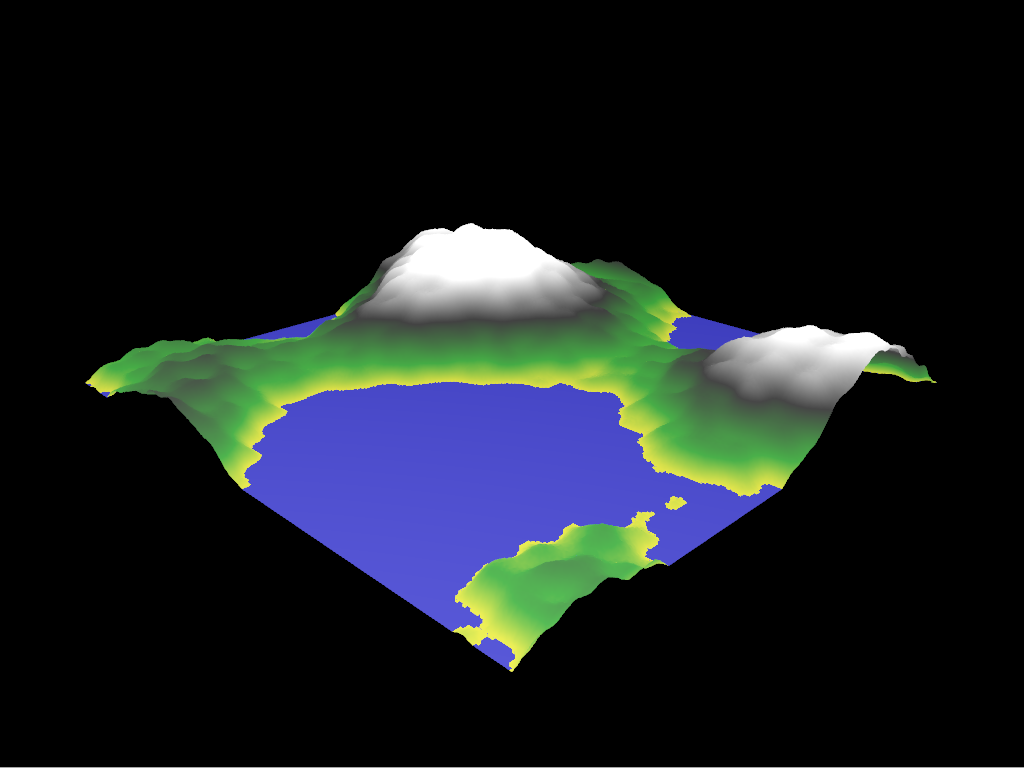
\includegraphics[height=3cm]{{{img_stage1/fBm_1.1_10.0_10_2.0_withZeroGrad_seed5}}}
	} 
	\subfloat[Seed of 8]{
		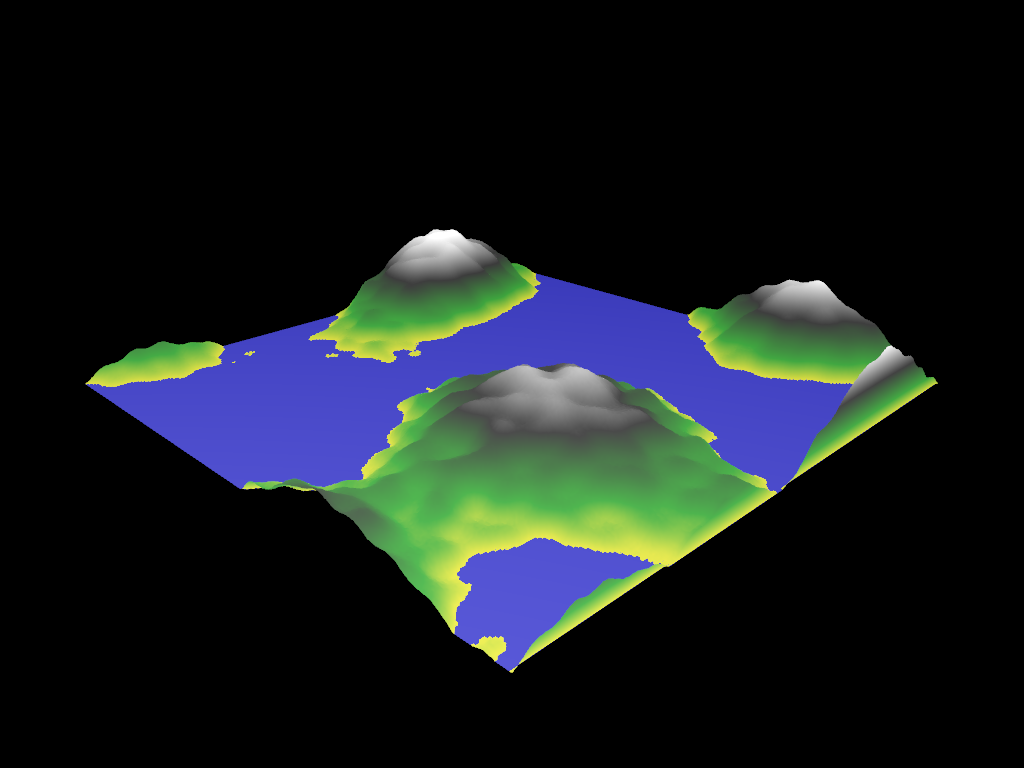
\includegraphics[height=3cm]{{{img_stage1/fBm_1.1_10.0_10_2.0_withZeroGrad_seed8}}}
	} 
	\subfloat[Seed of 10]{
		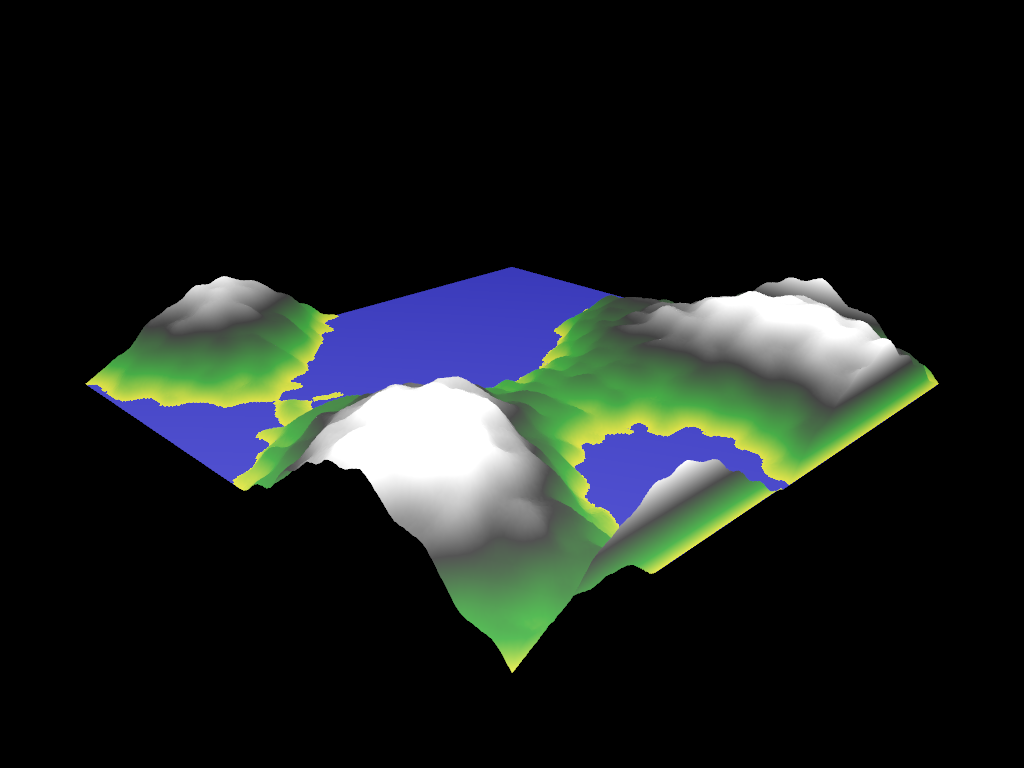
\includegraphics[height=3cm]{{{img_stage1/fBm_1.1_10.0_10_2.0_withZeroGrad_seed10}}}
	} \\
	\subfloat[Seed of 14]{
		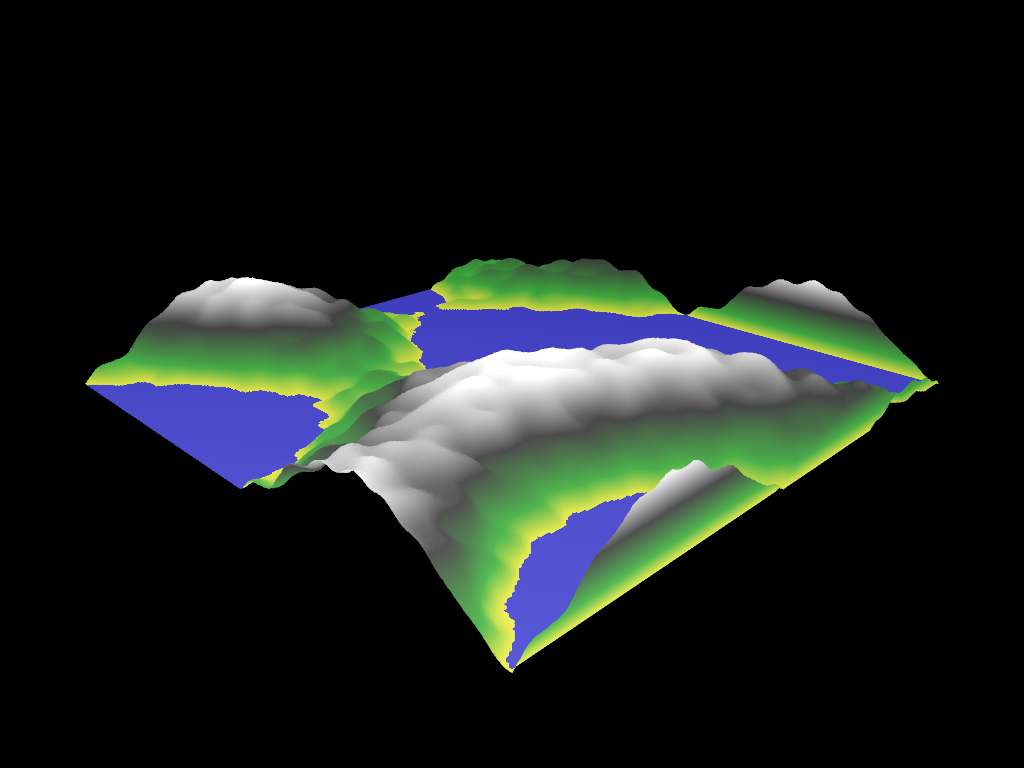
\includegraphics[height=3cm]{{{img_stage1/fBm_1.1_10.0_10_2.0_withZeroGrad_seed14}}}
	} 
	\caption{Example terrains generated by fractal Brownian motion with $H=1.1$, $l=10$ and 10 octaves, Perlin basis noise function. Different seeds were used to initialize the permutation table random shuffle.}
	\label{fBm}
\end{figure}

<<<<<<< HEAD
\subsection{Multifractal}

We implemented multifractal algorithm (equ.~\ref{eq_multifractal}) to generate a terrain using Perlin basis noise function or Simplec basis noise function. An example of such a generated terrain using Perlin and Simplex basis noise function are shown on figure ~\ref{multifractal}.

\begin{equation} \label{eq_multifractal}
	h = \prod\limits_{k=0}^{o} ( l^k \cdot \mathrm{perlin\_noise}(p) - off ) \cdot l^{-kH}
\end{equation}


\begin{figure}[ht]
	\centering
	\subfloat[Perlin noise basis]{
		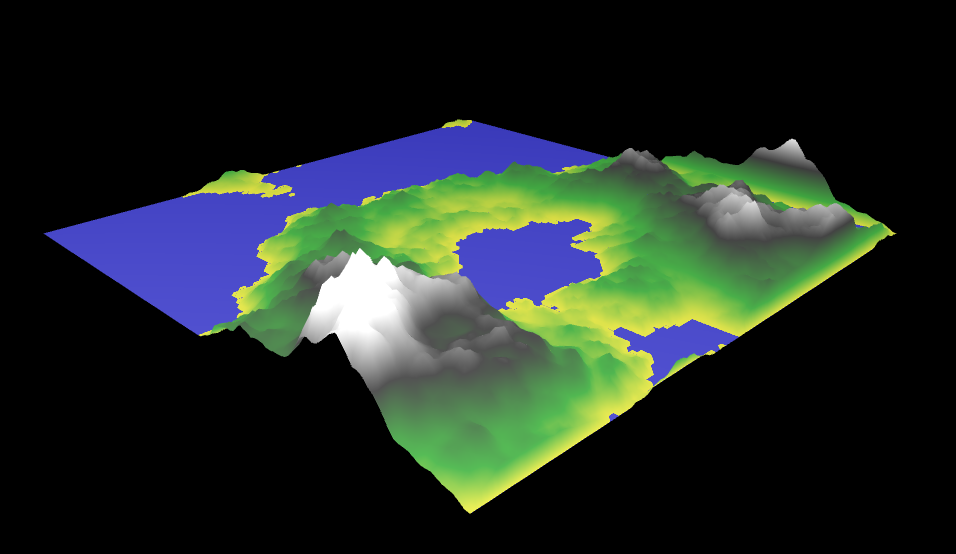
\includegraphics[height=4cm,width=6cm]{{{img_stage1/multifractal2}}}
	} \\
	\subfloat[Simplex noise basis]{
		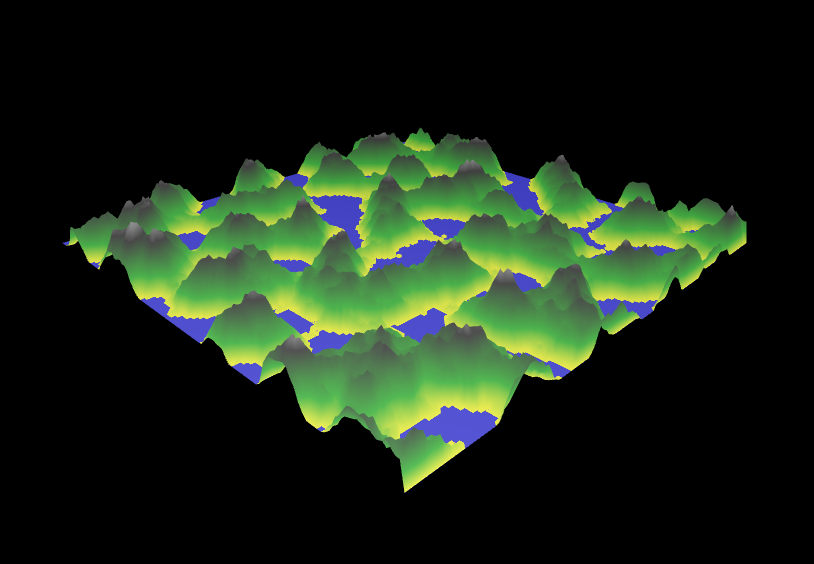
\includegraphics[height=4cm,width=6cm]{{{img_stage1/Multifractal_Simplex}}}
	} 
	\caption{Example terrain generated by multifractal}
	\label{multifractal}
=======
\subsection{Advanced topic : Multifractal}

\begin{figure}[ht]
	\centering
	\subfloat[Multifractal]{
		\label{multifractal}
		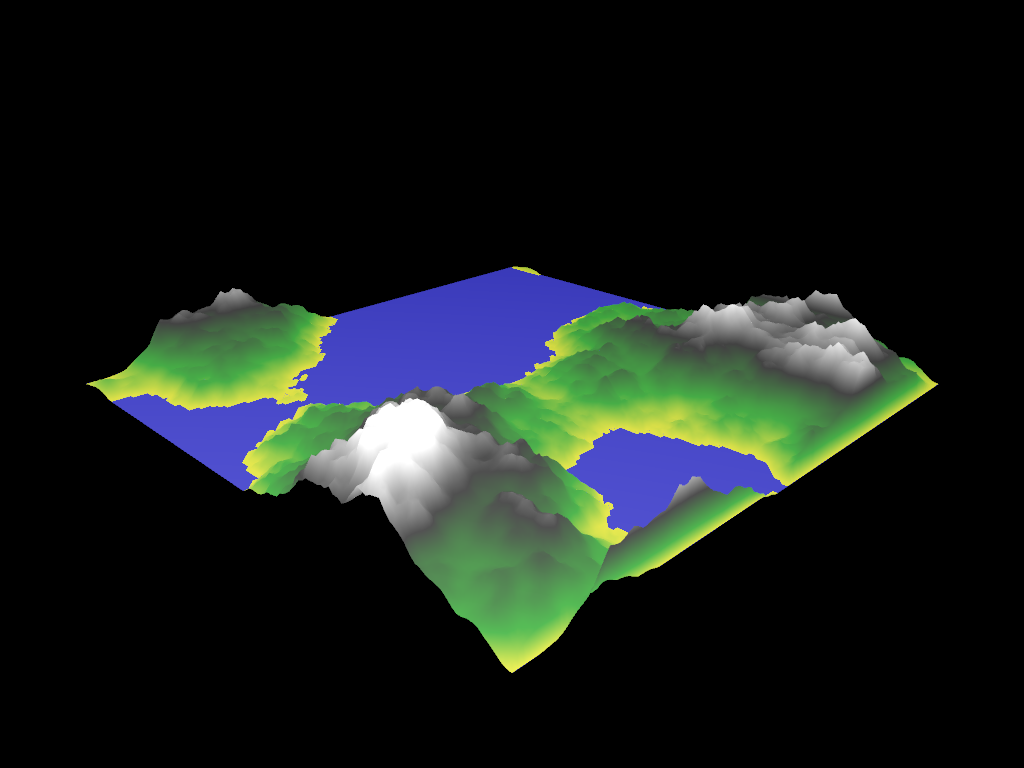
\includegraphics[height=4cm]{{{img_stage1/multifractal}}}
	} \quad
	\subfloat[Simplex noise]{
		\label{simplex_noise}
		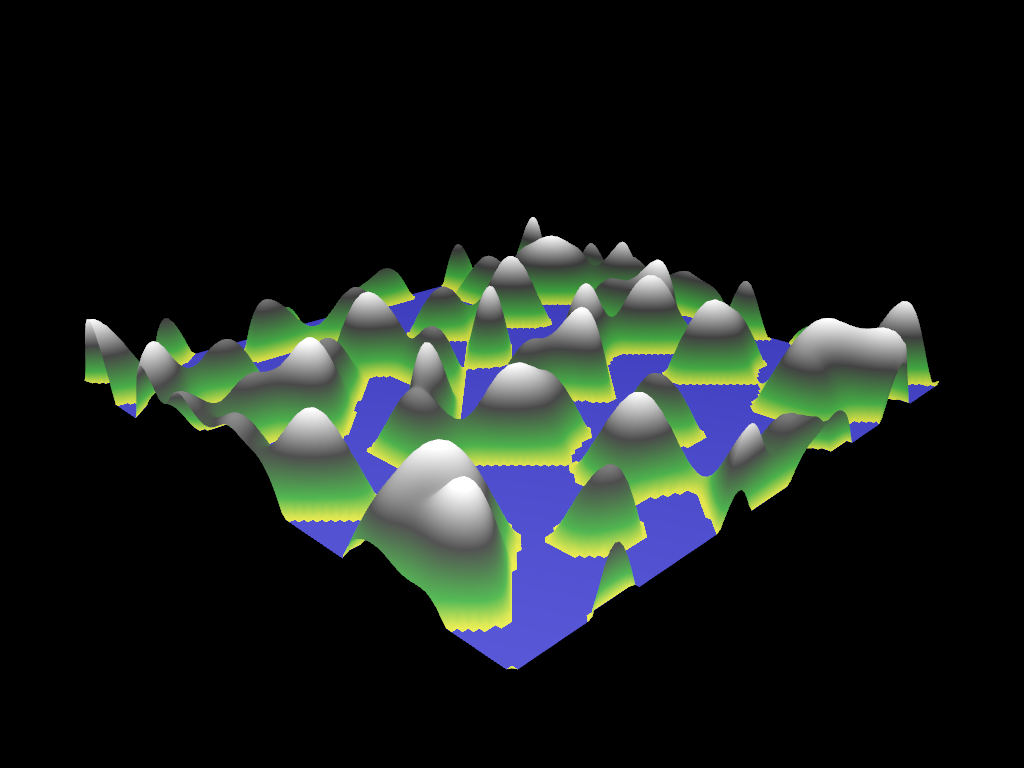
\includegraphics[height=4cm]{{{img_stage1/simplex_noise}}}
	}
	\caption{Example terrains}
	\label{terrain_examples}
>>>>>>> 318cf949ce05e2d98e6244c74a60bfba1a34eb34
\end{figure}

\subsection{Advanced topic : Simplex noise}

\section{Results}

Measure FPS

\end{document}
